\documentclass[10pt]{article}
\usepackage[margin=0.62in]{geometry}
\usepackage[hidelinks]{hyperref}
\usepackage{microtype}
\usepackage{tikz}
\usetikzlibrary{positioning,arrows.meta}
\setlength{\parindent}{0pt}
\setlength{\parskip}{0.35em}

\begin{document}

\begin{center}
{\large\textbf{Approach Writeup}}\\
\textbf{Fairness-Aware Sequential Decision-Making Under Uneven Context}\\
Piter Z. Garcia Bautista
\end{center}

\textbf{Approach Overview.}
This work proposes a shared framework for fairness-aware sequential decision-making in two target settings: clinical diagnostic workflows and quantum routing/resource allocation. The design is motivated by a common failure mode: decisions are made repeatedly under partial feedback, but the quality of the available context is not uniform across groups. In the clinical setting, that means some patients may be represented by weaker or delayed information during test selection or escalation. In the quantum setting, that means routing and resource-allocation decisions may be made under uncertain link quality, changing threats, and unequal access to scarce qubits. The contribution is therefore not simply ``using bandits in two places,'' but using one fairness-aware decision framework to test when richer context reduces disparity, when it only improves average utility, and when explicit mitigation is still required.

\begin{figure}[h]
\centering
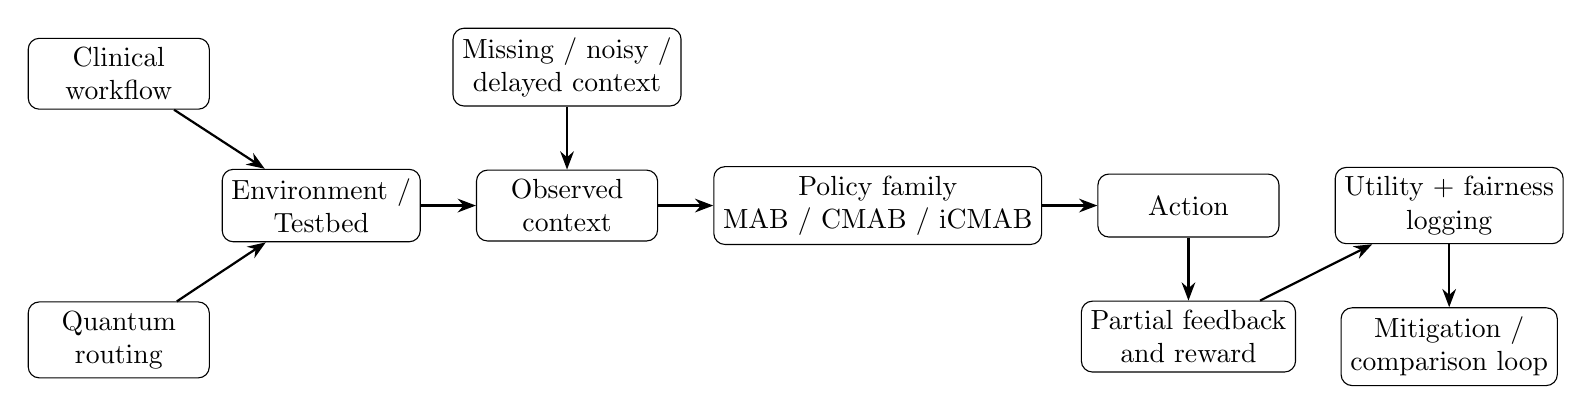
\begin{tikzpicture}[
box/.style={draw, rounded corners=4pt, align=center, minimum width=2.3cm, minimum height=0.8cm},
arr/.style={-Stealth, thick}
]
\node[box] (env) {Environment /\\Testbed};
\node[box, above left=0.75cm and 0.15cm of env] (clin) {Clinical\\workflow};
\node[box, below left=0.75cm and 0.15cm of env] (quant) {Quantum\\routing};
\node[box, right=0.7cm of env] (ctx) {Observed\\context};
\node[box, above=0.8cm of ctx] (deg) {Missing / noisy /\\delayed context};
\node[box, right=0.7cm of ctx] (pol) {Policy family\\MAB / CMAB / iCMAB};
\node[box, right=0.7cm of pol] (act) {Action};
\node[box, below=0.8cm of act] (fb) {Partial feedback\\and reward};
\node[box, right=0.7cm of act] (log) {Utility + fairness\\logging};
\node[box, below=0.8cm of log] (mit) {Mitigation /\\comparison loop};

\draw[arr] (clin) -- (env);
\draw[arr] (quant) -- (env);
\draw[arr] (env) -- (ctx);
\draw[arr] (deg) -- (ctx);
\draw[arr] (ctx) -- (pol);
\draw[arr] (pol) -- (act);
\draw[arr] (act) -- (fb);
\draw[arr] (fb) -- (log);
\draw[arr] (log) -- (mit);
\end{tikzpicture}
\caption{Shared domain model for the two testbeds. Both settings use the same fairness-aware sequential decision architecture while retaining different operational meanings and fairness metrics.}
\end{figure}

\textbf{Domain Model and Interaction Logic.}
Figure 1 shows the approach as a shared decision architecture rather than as two separate projects. Each testbed generates a decision state, exposes only the context that is available at that time, and then passes that observed context to a policy family spanning non-contextual, contextual, and informative-context bandit methods. The degradation mechanism is explicit because missing, noisy, or delayed context is part of the research question, not an implementation nuisance. The policy chooses an action, receives only bandit-style feedback for that action, and sends the resulting outcome to a logging layer that records both utility and fairness over time. This design allows the same interaction logic to support two distinct workflows: a clinical workflow where the action may be selecting a test or escalating follow-up, and a quantum workflow where the action may be choosing a path or allocating scarce routing resources. The domains remain separate, but the evaluation logic is shared.

\textbf{Why This Design.}
This design is stronger than several simpler alternatives. A single-domain study would be easier to communicate, but it would not test whether the same fairness-aware decision principles hold across technically different sequential systems. A contextual-only study would miss the point of the project, which is to compare a spectrum from non-contextual to contextual to informative-context methods and determine whether additional context actually improves fairness rather than only average performance. A post-hoc fairness audit would also be insufficient, because the central claim is that fairness must be measured during learning under partial feedback and shift. Finally, a vague generic framework plus a weak transfer story would repeat the earlier proposal problem; the architecture here is anchored in two concrete case studies that already have technical foundations. The simulation-first clinical design is intentional because it allows controlled experiments under missingness, noise, and shift without depending on sensitive patient data. The quantum testbed is credible because it builds on existing routing and resource-allocation work rather than inventing a second domain from scratch.

\textbf{Implementation Plan.}
The implementation follows directly from the domain model. First, a clinical simulation environment will model sequential decisions such as test ordering, retesting, or escalation when some groups have weaker observed context. Second, the existing quantum routing environment will be used to represent path selection and resource allocation under probabilistic link success and changing operating conditions. Both testbeds will expose the same policy interface so that multi-armed, contextual, and informative-context methods can be compared under shared logging and evaluation. The reward layer will track utility, cost, and latency, while the fairness layer will track domain-specific disparities such as clinical false-negative or delayed-escalation gaps and quantum service-equity gaps in success or latency across flow groups. At least one fairness-aware mitigation mechanism will then be evaluated inside the same framework. This approach is preferable to what has already been done because it makes the design decisions explicit, ties them to a common domain model, and tests fairness under uneven context as a first-class property of sequential decision systems rather than as an afterthought.

\begin{thebibliography}{9}\setlength{\itemsep}{0em}
\bibitem{li2010}
Li, L., Chu, W., Langford, J., and Schapire, R. A contextual-bandit approach to personalized news article recommendation. \textit{WWW}, 2010.
\bibitem{hardt2016}
Hardt, M., Price, E., and Srebro, N. Equality of opportunity in supervised learning. \textit{NeurIPS}, 2016.
\bibitem{joseph2016}
Joseph, M., Kearns, M., Morgenstern, J., and Roth, A. Fairness in learning: Classic and contextual bandits. \textit{NeurIPS}, 2016.
\bibitem{chen2020}
Chen, X., Zheng, A., Zhou, Z., and Shah, N. Fair contextual multi-armed bandits: Theory and experiments. \textit{UAI}, 2020.
\bibitem{garcia}
Garcia, P. Z. Threat-aware quantum routing via hybrid contextual bandits; and prior equitable bioinformatics work used as the clinical fairness foundation.
\end{thebibliography}

\end{document}
